\documentclass[a4paper,12pt,titlepage]{article}
\usepackage{palatino}
\usepackage{graphicx}
\usepackage{float}
\usepackage{amsmath}
\usepackage{caption}
\usepackage{subcaption}
\usepackage[margin=1.5cm,includefoot]{geometry}
\usepackage[utf8]{inputenc}
\usepackage{hyperref}
\usepackage{url}
\usepackage{listings}
\usepackage{xcolor}


\renewcommand*{\familydefault}{\sfdefault}

\usepackage[portuguese]{babel}

\begin{document}

	
	RFID, \textit{Radio Frequency Identification}, é uma tecnologia que está em crescente uso e discusssão atualmente, devido às suas possíveis aplicações e os benefícios que sua utilização propiciam. Seu principal uso é no monitoramento de ativos, permitindo conhecer toda a trajetória de um produto, desde o início da cadeia produtiva até o consumidor final. Avanços tecnológicos na fabricação de semicondutores permitiram tanto a redução do custo quanto a do tamanho dos componentes. Antes, as tags eram do tamanho de um forno-microondas e os leitroes construídos com antenas gigantescas. Hoje em dia, podemos encontrar leitores do tamanho de um moeda, e tags do tamanho de um grão de arroz, alavancando ainda mais a adoção da tecnologia RFID. Qualquer sistema de identificação no qual um dispostivo eletrônico usa radio frequência para o variações no campo magnético para comunicar e está anexado a um item, é definido como um RFID.
	
	Os dois principais componentes deste tipo de sistema são a \textit{Tag}, a qual é o dispositivo de identificação anexado ao item que desejamos monitorar, e o \textit{Leitor}, que é o dispositivo responsável por reconhecer as Tags e ler a informação contida nelas. O leitor pode então informar outros sistemas sobre a presença das tags, através de um \textit{RFID Middleware}. Este é um software que fornece a interface entre os leitores e o restante do sistema de informação. Na figura a seguir, podemos ver o sistema em questão:
	
	\begin{figure}[h!]
		\centering
		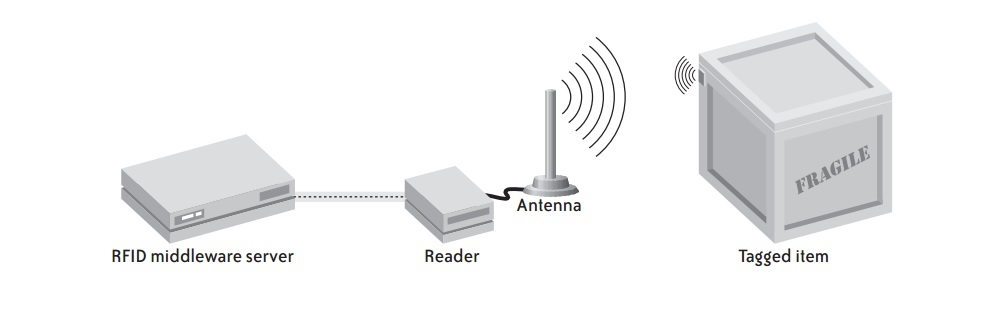
\includegraphics[width=0.6\linewidth]{rfidsys2}
		\caption{Sistema RFID típico, retirado de \cite{rfidbook}}
		\label{fig:rfidsys}
	\end{figure}
	
	Alguns dos benefícios do RFID são resumidos abaixo:
	\begin{itemize}
		\item Não há necessidade de alinhamento dos itens para leitura;
		\item Alta velocidade de inventário, pois vários itens podem ser lidos simultaneamente;
		\item Capacidade de identificar unicamente bilhões de itens;
		\item Variedade na forma das tags;
		\item Reusabilidade de tags.
	\end{itemize}
	
	\section{Evolução na adoção do RFID}
	De acordo com \cite{rfidbook}, podemos dividir o progresso de adoção do RFID em 5 períodos: \textit{Proprietary era}, \textit{Compliance era}, \textit{RFID-enable Enterprise era}, \textit{RFID-enable Industies era} e \textit{Internet of Things era}. A figura [\ref{fig:rfideras}] mostra quando algumas funções do RFID começaram ou vão começar a existir.
	
	\begin{figure}[h!]
		\centering
		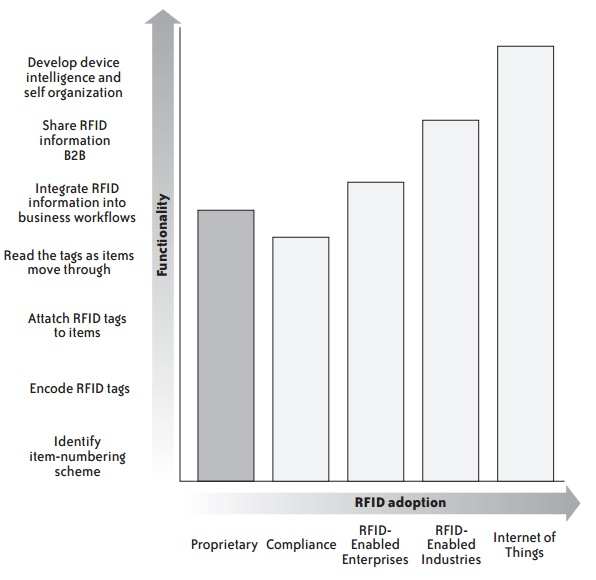
\includegraphics[width=0.6\linewidth]{rfideras}
		\caption{Evolução do RFID, retirado de \cite{rfidbook}}
		\label{fig:rfideras}
	\end{figure}
	
	No início (\textit{Proprietary era}), o RFID era usado para monitorar tipos particulares de itens e esta informação permanecia dentro das organizações que utilizavam o sistema. Isso fazia com que os sistemas fosse bastante específicos, dificultando bastante a comunicação entre parceiros de negócios. Alguns dos itens monitorados eram carros de trem, chassis de automóveis e gado leiteiro. Nesta época as tags ainda eram caras, logo estas eram reutilizadas sempre que possível. 
	
	Na \textit{Compliance era}, que representa o período atual, as empressas utilizam o RFID principalmente para garantir a interoperabilidade entre parceiros de negócios e agências regulatórias, não usando frequentemente os dados RFID para, por exemplo, aperfeiçoar alguns processos e melhorar a produtividade. A escassez de padrões e a falta de confiabilidade das novas tecnologias, impedem que as taga funcionem tão bem na prática como na época anterior.
	
	No futuro, teremos a \textit{The RFID-Enabled Enterprise era}, na qual as empresas começarão a utilizar as informações coletadas do RFID para o aprimoramento dos próprios processos. Isso será alcançado com a estabilização dos padrões e queda significativa dos custos. As empresas passarão a monitorar itens individuais ao invés de unidades de transporte, permitindo a coleta de mais informações sobre o processo. Entretanto, mesmo com a larga adoção interna do RFID, as empresas ainda precisam desenvolver os padrões necessários para permitir a troca de informações entre elas. 
	
	Em seguida teremos a \textit{The RFID-Enabled Industries era}, onde o uso de padrões RFID, redes de informação RFID, acordos de negócios e políticas de segurança e privacidade permitirão que empresas e cadeias de suprimentos troquem dados de forma segura e confiável entre si. Isso permitirá a descoberta de novas informações através do estudo  do grande volume de dados que estará disponível.   
	   
	Por fim, teremos a \textit{The Internet of Things era} que é atualmente uma previsão, na qual a ubiquidade da tecnologia RFID mudará a forma como vemos a relação entre informação, objetos físicos e localização. Por exemplo, a geladeira de nossa casa estará conectada à Internet e será capaz de ler a data de validade dos alimentos presentes e nos informar se algum deles já venceu. Além disso, ela poderá checar se algum produto está faltando e automaticamente realizar o pedido deste junto ao supermercado.
	
	A forma e velocidade com que os diversos tipos de usuários passarão por essas épocas não será feita de maneira uniforme. Atualmente, existem usuários que ainda estão na \textit{Proprietary era}, enquanto outros já estão começando a aplicar os conceitos da \textit{RFID-enabled Industries e Internet of Things}. Em algumas áreas, o RFID ainda nem começou a ser implementado.
	
	
	
	
	\newpage
	 \bibliographystyle{plain}
	 \nocite{*}
	 \bibliography{biblio_doc}
	 


\end{document}